\chapter{Related Theory}

\section{Introduction}
The development of a mobile application for the Institute of Engineering Purwanchal Campus (IOEPC) involves several theoretical concepts and technologies. This section explores the related theories and technologies that underpin the proposed solution, including mobile application development, monolithic architecture, MVVM architecture, and the use of React/React Native and Kotlin.

\section{Mobile Application Development}
Mobile application development refers to the process of creating software applications that run on mobile devices. This involves designing the user interface (UI), developing the backend services, and ensuring seamless integration between the frontend and backend components. The primary goal is to create a user-friendly and efficient application that meets the needs of its users (Smith, 2020).

\section{Monolithic Architecture}
A monolithic architecture is a software design pattern where all components of an application are integrated into a single, cohesive unit. This approach simplifies deployment and management, as all functionalities are contained within a single codebase. However, it can also lead to challenges in scalability and maintenance as the application grows (Johnson, 2019). For the proposed IOEPC application, a monolithic architecture is chosen for its simplicity and ease of deployment.

\begin{figure}[H]
    \centering
    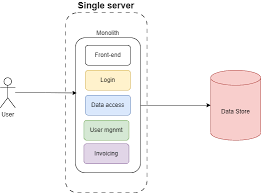
\includegraphics[width=0.8\textwidth]{Graphics/monolithic_architecture.png}
    \caption{Monolithic Architecture}
    \label{fig:monolithic_architecture}
\end{figure}

\section{MVVM Architecture}
Model-View-ViewModel (MVVM) is a software architectural pattern that facilitates the separation of the development of the graphical user interface (the view) from the development of the business logic or back-end logic (the model). The view model of MVVM is a value converter, meaning the view model is responsible for exposing (converting) the data objects from the model in such a way that objects are easily managed and presented. This pattern is particularly useful in mobile application development for maintaining a clean separation of concerns and enhancing testability (Garcia, 2020).

\begin{figure}[H]
    \centering
    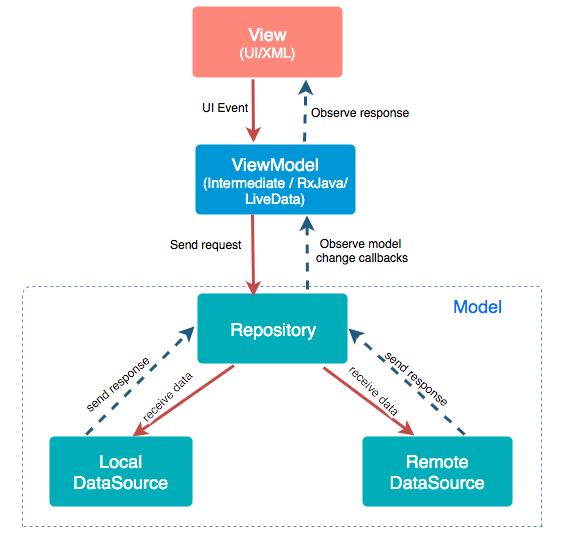
\includegraphics[width=0.8\textwidth]{Graphics/mvvm_architecture.png}
    \caption{MVVM Architecture}
    \label{fig:mvvm_architecture}
\end{figure}

\section{React/React Native}
React is a JavaScript library for building user interfaces, while React Native is a framework for building native mobile applications using React. Both technologies are widely used for their efficiency and flexibility in developing responsive and interactive UIs. React/React Native allows developers to create reusable components, which can significantly speed up the development process and ensure consistency across different parts of the application (Brown, 2018).

\section{Kotlin}
Kotlin is a modern programming language that is fully interoperable with Java and is officially supported for Android development. It offers several advantages over Java, including more concise syntax, improved safety features, and better support for functional programming. Kotlin is used for developing the student and teacher portals of the IOEPC application, providing a robust and efficient solution for Android devices (Lee, 2021).

\section{Conclusion}
The related theories and technologies discussed in this section form the foundation of the proposed mobile application for IOEPC. By leveraging the strengths of mobile application development, monolithic architecture, MVVM architecture, React/React Native, and Kotlin, the project aims to deliver a comprehensive and user-friendly solution that addresses the current challenges faced by the campus.